\documentclass{report}
\usepackage[utf8]{inputenc}
\usepackage[a4paper,margin=3cm,top=2cm]{geometry}
\usepackage{graphicx}
% graphics
\usepackage{tikz}
\usepackage{graphicx}
\usepackage{booktabs}
\usepackage{dirtree}
\usepackage{float}
\usepackage{tabularx}
\usepackage[indentafter]{titlesec}
\usepackage{xlop}
\usepackage{caption,subcaption}
\usepackage{setspace}
%listings
\usepackage{xcolor}
\usepackage{listings}
\lstdefinestyle{verilog}{
	backgroundcolor=\color{gray!10!white},
	basicstyle=\footnotesize\ttfamily,
	breaklines=true,
	commentstyle=\color{gray},
	escapeinside={~}{~},
	frame=single,
	keywordstyle=\color{blue},
	language=verilog,
	numbers=left,
	numbersep=5pt,
	showstringspaces=false,   
	numberstyle=\tiny\color{gray},
	rulecolor=\color{gray},
	stringstyle=\color{purple},
	tabsize=4}
\lstnewenvironment{code}{\lstset{style=verilog}\latin}{\endlatin}

\newcommand{\co}[1]{\lr{\lstset{style=verilog}\lstinline{#1}}}


\usepackage{fancyhdr}
\pagestyle{fancy}
\fancyhf{}
\fancyhead[LE,RO]{\leftmark}
\fancyhead[RE,LO]{مستند پروژه طراحی سیستم‌های دیجیتال}
\fancyfoot[LE,RO]{\thepage}

\onehalfspacing
% persian
\usepackage[extrafootnotefeatures,localise]{xepersian}
\settextfont[
Scale = 1.2]{XB Zar}
\setlatintextfont[Scale=1.2,
 BoldFont={LiberationSerif-Bold.ttf}, 
 ItalicFont={LiberationSerif-Italic.ttf}]{LiberationSerif-Regular.ttf}
 
\begin{document}

\begin{titlepage}
\newcommand{\HRule}{\rule{\linewidth}{0.1mm}} 
\center % Center everything on the page
 
%---------------------------------------------------------------------------------
%	HEADING SECTIONS (Enter the Homework/assignment No., only)
%---------------------------------------------------------------------------------
    \textsc{\Large دانشکده مهندسی کامپیوتر}\\[0.5cm] % heading course Number
    \textsc{\Large طراحی سیستم‌های دیجیتال}\\[0.5cm] % heading course name
    \textsc{\large مستند پروژه}\\[0.5cm] % Minor heading
%---------------------------------------------------------------------------------
%	TITLE SECTION (Replace 'TITLE' with the Homework/assignment Name/title)
%---------------------------------------------------------------------------------

\HRule \\[0.4cm]
    { \huge \bfseries  بررسی الگوریتم درهم‌سازی skein}\\[0.1cm] % Title of your Homework/assignment
\HRule \\[1.5cm]
 
%\maketitle
\begin{minipage}{0.4\textwidth}
\begin{center}

 \large
    
    \emph{نگارندگان:}\\
    حسن سندانی\\
    محمد صالح سعیدی\\
    مریم حکاک\\
    محمد مهدی عرفانیان\\
    علی جندقی
    \end{center}
\end{minipage}
\vspace{10mm}

{\large \today}\\[1cm] % Date, change the \today to a set date if you want to be precise

\includegraphics{figs/sharif.png}% \\[0.5cm] % 
\vfill % Fill the rest of the page with white-space
\end{titlepage}
\tableofcontents
\chapter{مقدمه}
\noindent
\textbf{
\textit{
توضیحی اولیه مشتمل بر تعریف الگوریتم، نحوه کلی عملکرد الگوریتم، پایه‌های ریاضی، کاربردها و استانداردها
}
}
\pagebreak
\section{توضیح الگوریتم}
\par
الگوریتمی که در ادامهٔ این مستند شرح و توضیح آن آمده است الگوریتم درهم سازی 
\lr{skein}
یا 
\lr{skein hash function}
است. این الگوریتم از سری الگوریتم‌های درهم‌سازی امنیتی یا 
\lr{cryptographic hash function}
 و یکی از نامزدهای نهایی مسابقه انتخاب بهترین تابع درهم‌سازی 
 \lr{NIST}
 می‌باشد. این مسابقه برای انتخاب بهترین الگوریتم در‌هم‌سازی برای استاندارد جدید 
 \lr{SHA-3}
 برگزار شد. 
 طبق ادعای طراحان الگوریتم این الگوریتم می‌تواند در 
 \lr{6.1}
 کلاک در بایت داده‌ها را هش کند، که به این معنیست که در پردازندهٔ دوهسته‌ای
 \lr{64}
  بیتی با فرکانس پردازشی
\lr{3.1 GHz}
    می‌تواند با سرعت 
\lr{500}
  مگابایت بر ثانیه داده‌ها را هش کند. این مقدار سرعت تقریبا دوبرابر سرعت هش کردن دادهٔ الگوریتم 
  \lr{ SHA-512}
  است. همچنین با گزینه درخت درهم‌سازی که می‌تواند به صورت اختیازی در الگوریتم پیاده‌سازی شود می‌توان 	در پیاده‌سازی موازی الگوریتم سرعت را به بیش از این هم رساند. نکته دیگری که در مورد الگوریتم 
  \lr{skein}
  لازم به ذکر است این است که این الگوریتم پیاده‌سازی آسان و ساده‌ای دارد و فقط از سه عمل‌گر اصلی برای محاسبه هش استفاده می‌کند و نحوهٔ عملکرد الگوریتم به راحتی قابل به خاطرسپاری و یادگیری‌ست. 
  \par
  الگوریتم درهم‌سازی
  \lr{skein}
  برای حالت‌های ورودی ۲۵۶، ۵۱۲ و ۱۰۲۴ بایتی و هرمقداری خروجی پیاده‌سازی شده است که این خاصیت در انعطاف الگوریتم در حالت‌های مختلف بسیار حیاتی‌ست. 
  \\
  در پیاده‌سازی سخت‌افزاری نیز این الگوریتم قوی عمل می‌کند،‌برای پیاده‌سازی 
  \lr{skein-512}
  بر سخت‌افزار به حدود ۲۰۰ بایت فضای مموری نیاز داریم، برای 
  \lr{skein-256}
  این مفدار به حدود ۱۰۰ بایت کاهش پیاده می‌کند که این الگوریتم را به یک الگوریتم مناسب برای پیاده‌سازی‌های روی قطعات کوچک سخت‌افزاری تبدیل می‌کند، مثلا می‌توان از 
  \lr{skein-256}
  در پیاده‌سازی 
  \lr{smart card}
  استفاده کرد.
  \cite{skein}
 
  
  \subsection{مثال‌هایی از درهم‌سازی}

	\begin{itemize}
	
	\item \lr{Skein-256-256("")}\\
$c8877087da56e072870daa843f176e9453115929094c3a40c463a196c29bf7ba$
\item \lr{Skein-512-256("")}\\
$39ccc4554a8b31853b9de7a1fe638a24cce6b35a55f2431009e18780335d2621$
\item \lr{Skein-512-512("")}\\
$bc5b4c50925519c290cc634277ae3d6257212395cba733bbad37a4af0fa06af4$\\
$1fca7903d06564fea7a2d3730dbdb80c1f85562dfcc070334ea4d1d9e72cba7a$

	\end{itemize}
	
\section{مختصری دربارهٔ الگوریتم‌های درهم‌سازی امنیتی}
در دنیای امروز الگوریتم‌های درهم‌سازی امنیتی تقریبا در تمامی نقاط مختلفی که با اینترنت سر و کار دارند پیدا می‌شوند، بزرگ‌ترین کاربرد این الگوریتم‌ها ایجاد امضای دیجیتالی یا 
\lr{digital signature}
است که در ذخیرهٔ رمزهای عبور، اتصالات امنیتی به سرورها، مدیریت رمزنگاری‌ها و اسکن ویروس‌ها و بدافزارها به کار می‌رود، تقریبا تمامی پروتکل‌های امنیتی در دنیای اینترنت امروز بدون الگوریتم‌های درهم‌سازی امنیتی به سختی قابل پیاده‌سازی خواهند بود. 
\par
بزرگترین الگوریتم‌های درهم‌سازی امنیتی فعلی الگوریتم‌های خانواده 
\lr{SHA}
می‌باشند، الگوریتم‌های خانواده 
\lr{SHA}
به اختصار نام موارد زیر اند.
\begin{itemize}
\item
	\lr{SHA-0}
	\item
	\lr{SHA-1}
	\item
	\lr{SHA-256}
	\item
	\lr{SHA-512}
\end{itemize}
تمامی موارد بالا از روی الگوریتم‌های 
\lr{MD4} 	و
\lr{MD5}
اقتباس شده اند. 
در سال‌های اخیر کاستی‌ها و مشکلات امنیتی زیادی در الگوریتم‌های 
\lr{MD4, MD5, SHA-0, SHA-1}
یافت شدند اما هنوز باگ امنیتی بزرگی برای الگوریتم‌های 
\lr{SHA-256, SHA-512}
یافت نشده است اما به دلیل وابستگی زیاد صنعت و امنیت فعلی اطلاعات به الگوریتم‌های درهم‌سازی در سال ۲۰۱۲ 
تصمیم بر این شد تا جایگزین مناسب و جدیدی برای الگوریتم‌های 
\lr{SHA-256, SHA-512}
انتخاب شود تا در صورتی که این الگوریتم‌ها شکسته شدند به سرعت الگوریتم‌های جدید در قالب نام 
\lr{SHA-3}
جایگزین شوند. 
\section{هدف الگوریتم درهم‌سازی skein}	
هدف الگوریتم درهم‌سازی skein مانند دیگر الگوریتم‌های درهمسازی امنیتی ایجاد یک تابع برای درهم‌سازی داده‌های مختلف است به شکلی که ویژگی‌ها زیر برای آنان برقرار باشند.

\begin{itemize}
\item قطعی بودن:
به شکلی که به ازای ورودی یکسان مقدار در‌هم‌سازی با تکرار الگوریتم برابر باشد، مثلا با دادن ورودی "salam" به صورت متوالی به تابع مقدار هش تغییر نکند. 
\item یک طرفه بودن:
نتوان از مقدار خروحی مقدار ورودی را یافت. 
\item
یک به یک بودن:
نتوان دو ورودی پیدا کرد به شکلی که به ازای این دو ورودی مقدار خروجی مساوی شود.
\item حساس بودن:
با تغییر اندک در ورودی خروجی به شکل قابل ملاحظه‌ای تفییر کند تا مقدار هش قابل حدس زدن نباشد.
\item
سریع بودن: 
الگوریتم باید بتواند هش را در مدت زمانی کوتاهی حساب کند تا به کاربردی بودن برسد.

\end{itemize}


\section{نحوهٔ کلی عملکرد الگوریتم}
ایدهٔ اصلی الگوریتم بر ایجاد بلوک‌های زمزگذاری قابل تنظیم یا به زبان نویسندگان الگوریتم
\lr{tweakable block cipher}
بنا نهاده شده است؛ به صورت دقیق‌تر می‌توان گفت که
Skein 
از سه قسمت اصلی زیر تشکیل شده است و برای درهم‌سازی از ایشان استفاده می‌کند.
\begin{itemize}
\item
\lr{\textbf{Threefish}}\\
این قسمت یک بلوک رمزگذاری قابل تنظیم است که در هسته اصلی الگوریتم پیاده‌سازی شده است، این بلوک‌ها در سایزهای ۲۵۶، ۵۱۲، ۱۰۲۴ بیتی تعریف شده اند.
\item
\lr{\textbf{Unique Block Iteration (UBI)}}\\
\lr{UBI}
یک حالت زنجیری‌ست که با استفاده از بلوک قبلی به عنوان ورودی خود سعی در ایجاد یک الگوریتم فشرده‌سازی مخصوص ورودی می‌کند که بلوک ورودی با سایز دلخواه را به یک خروحی با سایز مشخص تبدیل کند.
\item
\lr{\textbf{Optional Argument System}}\\
این ویژگی به الگوریتم اجازه می‌دهد تا از تعدادی ویژگی اختیاری بدون تحمیل هزینه بیش از حد اجرایی استفاده کند. 
\cite{main_doc}
\end{itemize}
	
\begin{thebibliography}{1}


\bibitem{skein}{
\lr{
http://www.skein-hash.info/about\\
  }}
  
  \bibitem{main_doc}
  \lr{The Skein Hash Function Family\\
Version 1.3 — 1 Oct 2010\\
http://www.skein-hash.info/sites/default/files/skein1.3.pdf\\
}
  
\end{thebibliography}

\chapter{توصیف معماری سیستم}
\noindent
\textbf{
	\textit{
		تشریح اینترفیس‌های سیستم، کلاک‌ها و نحوهٔ راه‌اندازی سیستم، دیاگرام بلوکی سخت‌افزار، ساختار درختی سیستم و توصیف ماژول‌های سخت‌افزار 
	}
}
\pagebreak

\section{ اینترفیس‌های سیستم}
در ابتدا به صورت خلاصه اینترفیس‌های سیستم سخت‌افزاری الگوریتم Skein بیان می‌شود، اینترفیس یک سیستم شامل ورودی‌ها و خروجی‌ها و مشخصات ایشان است. 
\subsection{ورودی‌ها}
ورودی‌ها کد verilog الگوریتم Skein به شرح زیر اند.
\begin{itemize}
	\item
	      \textbf{clk}\\
	      ورودی کلاک سیستم است که با آن سیستم کار خود را به صورت ترتیبی 
	      \footnote{\lr{Sequential}}
	      انجام می‌دهد، فرکانس کلاک با توجه به نحوهٔ پیاده‌سازی سخت‌افزاری و نتایج حاصل از سنتز تعیین می‌شود. در Testbench داده شده کلاک هر ۱۰ نانوثانیه تغییر می‌کند.
	\item
	      \textbf{\lr{midstate}}\\
	      ورودی ۵۱۲ بیتی برای الگوریتم
	      \lr{Skein-512}
	      است که حالت میانی در هش را معلوم می‌کند.
	\item
	      \textbf{nonce}\\
	      nonce مقداری دلخواه است که برای به حداکثر رساندن تصادفی  و غیرقابل شکستن بودن هش 
	      در محاسبه هش استفاده می‌شود، این مقدار می‌تواند عددی دلخواه باشد. در الگوریتم 
	      \lr{Skein-512}
	      اندازهٔ این ورودی ۳۲ بیت به اندازه طول عدد در Integer گرفته شده است.
	\item
	      \textbf{data}\\
	      ورودی اصلی‌ست که باید هش آن محاسبه شود، در کد verilog داده شده اندازه این ورودی ۹۶ بیت در نظر گرفته شده است. 
\end{itemize}

\subsection{خروجی}
تنها خروجی سیستم مقدار هش در output است که ۵۱۲ بیت طول دارد.
(الگوریتم مورد بحث 
\lr{Skein-512}
است)

\section{کلاک‌ها و نحوهٔ راه‌اندازی سیستم}
این سیستم فقط از یک کلاک استفاده می‌کند و برای راه‌اندازی سیستم انجام کارهای زیر ضروری‌ست.
\begin{enumerate}
	\item
	      وصل کردن کلاک با فرکانس مناسب به سیستم
	\item
	      اعمال ریست‌ کلی بر سیستم
	      \footnote{\lr{Global Reset}}
	\item 
	      تعیین ورودی‌های اولیه 
	\item 
	      راه‌اندازی سیستم 
\end{enumerate}


\section{دیاگرام بلوکی سخت‌افزار}
دیاگرام بلوکی کلی سخت‌افزار در شکل 
\ref{block_diagram}
آمده است. 

\begin{figure}
	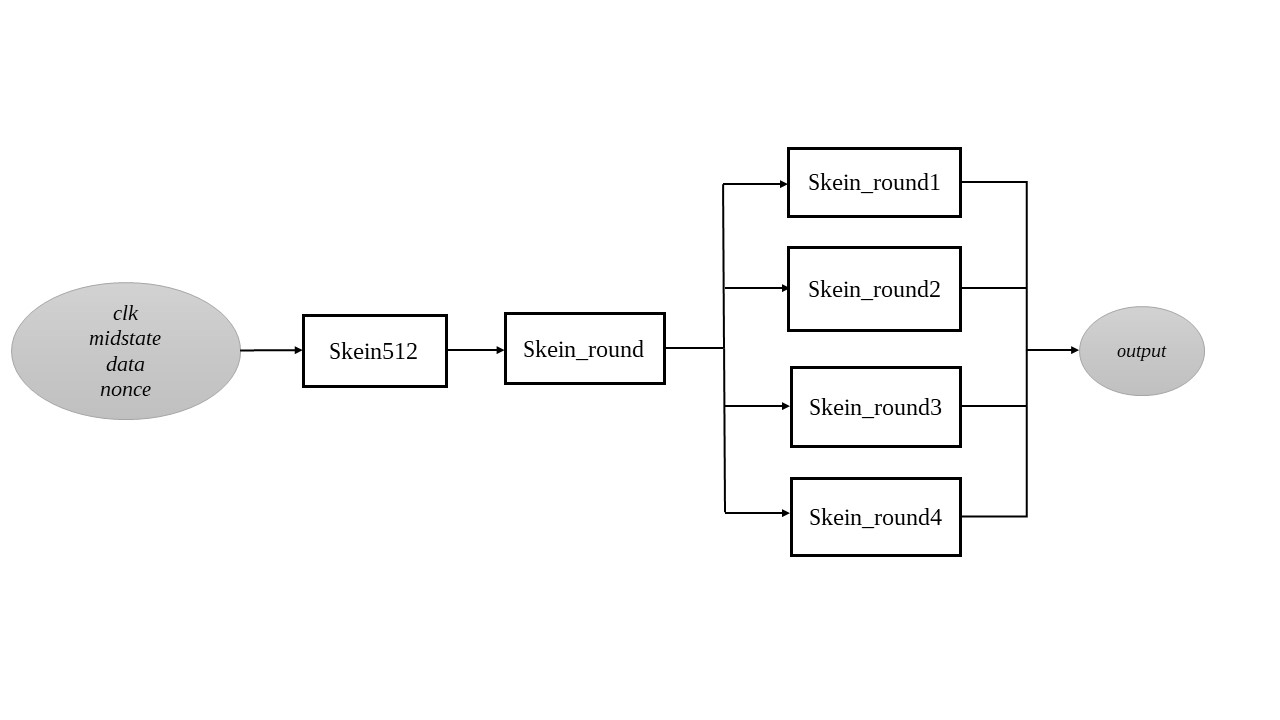
\includegraphics[width = \textwidth]{figs/DescriptionOfSystem/block_diagram.jpg}
	\caption{دیاگرام بلوکی سخت‌افزار}
	\label{block_diagram}
\end{figure}

\section{توصیف ماژول‌های سخت‌افزار}
\subsection{\lr{Skein-512}}
\subsubsection{اطلاعات کلی}
\lr{
\begin{table}[H]
\centering
\begin{tabular}{@{}ll@{}}
\toprule
\multicolumn{2}{l}{skein512}                                           \\ \midrule
$clk, {[}511:0{]} midstate, {[}95:0{]} data, {[}31:0{]} nonce$ & inputs  \\
${[}511:0{]} hash $                                            & outputs \\ \bottomrule
\end{tabular}%
\rl{
\caption{اطلاعات کلی ماژول \lr{skein512}}}
\label{table_skein512}
\end{table}}
درخطوط اولیه تعداد reg و wire تعریف شده است.
دو reg به نام های$ phase\_d$ و $phase\_q $تعریف شده اند که یک‌بیتی اند و مقدار صفر به آنها داده شده است.\\
دو assignment یک‌خطی دیده می‌شود.

\begin{enumerate}
	\item در reg 32 بیتی با نام $nonce\_le$ که در خطوط بالاتر تعریف شده است مقادیر $nonce$ (که ورودی 32 بیتی ماژول هستند) به صورت 8 بیت – 8 بیت و به صورت برعکس ذخیره می‌شوند. یعنی به طور مثال 8 بیت کم ارزش\  $nonce$در 8 بیت پرارزش $nonce\_le$ ذخیره شده اند.
	      
	\item در reg 32 بیتی با نام $nonce2\_le$ که در خطوط بالاتر تعریف شده است مقادیر $nonce2$ (که برعکس $nonce$، ورودی ماژول نیست و خود در خطوط بالاتر به صورت یک reg 32 بیتی تعریف شده است و در واقع در حال حاضر مقداری را به خود اختصاص نداده است) به صورت 8 بیت – 8 بیت و به صورت برعکس ذخیره می‌شوند. یعنی به طور مثال 8 بیت کم ارزش\  $nonce2$در 8 بیت پرارزش  $nonce2\_le$ ذخیره شده اند. (خط 56)
\end{enumerate}

یک عبارت assign طویل مربوط به hash دیده می‌شود:

\begin{itemize}
	\item
	      در این عبارت بیت‌های reg ی به نام
	      h\_q 
	      که 512 بیت دارد و در خطوط بالاتر تعریف شده است، به بیت های خروجی hash اساین می‌شود.
	\item
	      64 مجموعه 8 بیتی از $h\_q$ به بیت های hash اساین می‌شود که نظم این مقداردهی در زیر توضیح داده می‌شود. در این توضیحات hash را به ترتیب از پرارزش‌ترین ۸ بیت شروع به پر کردن میکنیم.
	\item
	      پرارزش‌ترین بیت‌های hash با بیت های $463$ تا $456$ پر شده است. (یعنی پرارزش ترین بیت hash با بیت $463$ ام $h\_q$ پر شده است و به همین ترتیب)
	\item
	      مجموعه بعدی 8 تایی از$464$ تا $471$ هستند که در دومین 8 تایی با ارزش hash قرار می‌گیرند.
	\item
	      این روند تا هشتمین 8 بیت ارزشمند hash ادامه پیدا میکند جایی که در این جایگاه مجموعه $[511:504]$ از $h\_q$ جای میگیرد. (تا اینجا نظم داشتیم)
	\item
	      نهمین 8 بیت ارزشمند hash توسط بیت های $[391:384]$ از $h\_q$ پر میشوند.
	\item
	      این روند ادامه پیدا میکند (یعنی دهمین 8 بیت ارزشمند با $[399:392]$ پر میشوند).
	      تا 16امین 8 بیت ارزشمند hash که با مجموعه $[447:440]$ پر شده اند.
	\item
	      17امین 8 بیت ارزشمند با مجموعه $[327:320]$ پر میشود.
	\item
	      این روند مانند قبل به صورت صعودی ادامه پیدا خواهد کرد تا به 25 امین مجموعه 8 بیتی برسیم.
	      
\end{itemize}

\textit{\textbf{درواقع هر 8 بار که مجموعه بیت های 8 بیتی را assign میکنیم، یک بی‌نظمی داریم.
}}
\begin{itemize}
	\item
	      25 امین 8 بیتی hash با بیت های $[263:256]$ پر میشود.
	\item
	      دوباره روند سابق و صعودی را داریم تا به 33 امین assignment برسیم.
	\item
	      33 امین 8 بیتی hash با بیت های $[199:192]$
	      
\end{itemize}

\textit{\textbf{هر بار بی‌نظمی داریم بازه جدید بعد از بی نظمی 120 واحد کمتر از بازه قبلی خواهد بود مثلا 32 امین 8بیت پرارزش hash با بیت های $[319:312] $پر شده اند که 120 واحد از بازه ای که برای 33امین 8 بیت ارزشمند hash اختصاص داده میشود بیشتر است. (در بالا 33امین نوشته شده است)}}

\begin{itemize}
	\item
	       8 مجموعه که به صورت صعودی پیش برویم به 40 امین 8بیت میرسیم که طبق نظم با بیت های $[255:248]$ پر شده است و 41امین 8 بیتی با بازه $[135:128]$ پر شده است.
	\item
	       8 مجموعه که به صورت صعودی پیش برویم به 48 امین 8بیت میرسیم که طبق نظم با بیت های $[191:184]$ پر شده است و 49امین 8 بیتی با بازه $[71:64]$ پر شده است.
	\item
	       8 مجموعه که به صورت صعودی پیش برویم به 56 امین 8بیت میرسیم که طبق نظم با بیت های $[127:120]$ پر شده است و 57امین 8 بیتی با بازه $[7:0]$ پر شده است.
	\item
	      از 57 امین مجموعه 8 تایی با ارزش hash تا آخرین مجموعه باارزش hash (64 امین) نیز به صورت صعودی و طبق نظم پیش میرود. (خط 121)
	      
\end{itemize}

بعد از خطوط 
assignment،
 ۱۸ instance از ماژول skein\_round گرفته شده است.
این instance ها را از 
$00$
تا
$0H$
نام گذاری کردیم (نامگذاری در مبنای بالاتر از 10 شده است)

\subsubsection{
	ورودی skein\_round ها
}
\begin{itemize}
	\item
	      \textbf{کلاک}
	      که همه به کلاک سیستم متصل اند.
	\item
	      \textbf{Round}
	      رجیستر 32 بیتی که به ترتیب ورودی 0 تا 17 به هر اینستنس داده شده است.
	\item
	      \textbf{$\textbf{p}$} 
	      رجیستر 512 بیتی – که به اینستنس شماره $01$ تا $0H$ به ترتیب $p01$ تا $p0H$ وصل شده است. به اینستنس شماره $00$ هم $p00\_q$ وصل شده است.
	\item
	      \textbf{$\textbf{H}$}
	      رجیستر 576 بیتی – که به اینستنس شماره $01$ تا $0H $به ترتیب $h01$ تا $h0H$ وصل شده است. به اینستنس شماره $00$ هم $h00\_q$ وصل شده است.
	\item
	      \textbf{$\textbf{T0}$}
	      رجیستر 64 بیتی –   که به اینستنس شماره $00$ تا $0H$ به ترتیب این دنباله 3 تایی وصل شده است:
	      $t0\_q, t1\_q, t2\_q$
	      این دنباله 3 جمله ای به ترتیب تکرار میشود.
	\item
	      \textbf{$\textbf{T1}$}
	      رجیستر 64 بیتی – دقیقا مثل $T0$ با این تفاوت که دنباله 3 تایی $ t1\_q، t2\_q, t0\_q $ به این شکل است.
	\item
	      \textbf{$\textbf{P0}$}
	      رجیستر 512 بیتی- که اینستنس شماره $00$ تا $0H$به ترتیب $o00$ تا $o0H$ وصل شده است. 
	\item
	      \textbf{$\textbf{H0}$}
	      رجیستر 576 بیتی- که اینستنس شماره $00$ تا $0H $به ترتیب $ho00 $تا $ho0H$ وصل شده است. خط(141)
	      
\end{itemize}
\textit{\textbf{
	در ادامه یک always بلاک داریم که حساس به تغییرات همه چیز است. (خط 143)
	در این بلاک متغیر هایی که در انتهایشان
	\_d
دارند مقداردهی میشوند.}}\\
ابتدا phase\_d مقدار not متغیر phase\_q را به خود اختصاص میدهد.
\begin{itemize}
	\item
	      \textbf{اگر phase\_q یک باشد}
	      \begin{itemize}
	      	\item
	      	      مقداردهی به $p00\_d$ (512 بیتی): 64 بیت کم ارزش ( $[63:0]$) از data در 64 بیت پرارزش $p00\_d$ قرار میگیرد. سپس در 32 بیت بعدی $p00\_d$ (از چپ) عینا nonce\_le قرار داده میشود. سپس 32 بیت باقیمانده از $data ([95:64])$ طبق روند قرار داده میشود. باقی بیت های این رجیستر هم با صفر پر میشوند $(384'd)$ – (خط 148)
	      	\item
	      	      مقداردهی به$ h00\_d$ (576 بیتی): در 64 بیت کم ارزش این reg مقدار صفر قرار داده میشود و باقی بیت ها دقیقا به midstate (ورودی 512 بیتی) متصل میشوند.
	      	\item
	      	      مقداردهی به$ t0\_d$ (64 بیتی) : $h0000000000000050$
	      	\item
	      	      مقداردهی به$ t1\_d$ (64 بیتی) : $hb000000000000000$
	      	\item
	      	      مقداردهی به $t2\_d$ (64 بیتی) : $hb000000000000050$
	      	\item
	      	      h\_d هم مقدار h\_q را به خود میگیرد.
	      \end{itemize}
	\item
\textbf{	      اگر phase\_q صفر باشد
}	      \begin{itemize}
	      	\item
	      	      مقداردهی به $p00\_d$ (512 بیتی): این reg با صفر پر میشود.
	      	\item
	      	      مقداردهی به $h00\_d$ (576 بیتی):
	      	      \begin{itemize}
	      	      	\item
	      	      	      بیت های $[575:512]$:	
	      	      	      	$data[63:0] \textasciicircum ( oH[511:448] + hH[575:512])$
	      	      	\item
	      	      	      بیت های $[511:448]$: 
	      	      	      	\{ $nonce2\_le$ , $data[95:64$ \} \textasciicircum ( $oH[447:384] + hH[511:448]$)
	      	      	\item
	      	      	      بیت های $[447:384]$:  $	oH[383:320] + hH[447:384]$
	      	      	\item
	      	      	      بیت های $[383:320]$:$	oH[319:256] + hH[383:320]$
	      	      	\item
	      	      	      بیت های $[319:256]$:$	oH[255:192] + hH[319:256]$
	      	      	\item
	      	      	      بیت های $[255:192]$:
	      	      	      $	oH[191:128] + hH[255:192] + 
	      	      	      64'h0000000000000050$
	      	      	\item
	      	      	      بیت های $[191:128]$:	
	      	      	      $oH[127: 64] + hH[191:128] + 64'hb000000000000000$
	      	      	\item
	      	      	      بیت های $[127:64]$:
	      	      	  $    	oH[ 63:  0] + hH[127: 64] + 18$
	      	      \end{itemize}
	      	\item
	      	      مقداردهی به$ t0\_d$ (64 بیتی) : $h0000000000000008$
	      	\item
	      	      مقداردهی به $t1\_d$ (64 بیتی) : $hFF00000000000000$
	      	\item
	      	      مقداردهی به $t2\_d$ (64 بیتی) : $hFF00000000000008$
	      	\item
	      	      مقداردهی به $h\_d$ (512 بیتی):
	      	      \begin{itemize}
	      	      	\item
	      	      	      بیت های $[511:448]$:
	      	      	      $ 	o0H[511:448] + ho0H[575:512]$
      	      	    \item
	      	      	      بیت های $[447:384]$:  
	      	      	      	$o0H[447:384] + ho0H[511:448]$
	      	      	\item
	      	      	      بیت های $[383:320]$:
	      	      	      $	o0H[383:320] + ho0H[447:384]$
	      	      	\item
	      	      	      بیت های $[319:256]$:
	      	      	      $	o0H[319:256] + ho0H[383:320]$
	      	      	\item
	      	      	      بیت های $[255:192]$:
	      	      	      $	o0H[255:192] + ho0H[319:256]$
	      	      	\item
	      	      	      بیت های $[191:128]$:	
	      	      	      $o0H[191:128] + ho0H[255:192] + 64'h0000000000000008$
	      	      	\item
	      	      	      بیت های $[127:64]$:	
	      	      	      $o0H[127: 64] + ho0H[191:128] + 64'hFF00000000000000$
	      	      	\item
	      	      	      بیت های $[63:0]$:	
	      	      	      $	o0H[ 63:  0] + ho0H[127: 64] + 18$
	      	      	 
	      	      \end{itemize}
	      \end{itemize}
\end{itemize}
\textit{
	\textbf{نظم مناسبی دیده میشود به این شکل که به ترتیب 64 بیت پرارزش h\_d با مجموع 64 بیت پرارزش $o0H$ و 64 بیت پرارزش $ho0H$ پر میشود. به جز 3 مورد آخر که با اعدادی ثابت هم جمع میشوند.
}}\\

\textit{\textbf{Always بلاک دوم فقط به لبه مثبت کلا384’ک حساس است. (خط 211)
	(عموما متغیر های \_q، مقادیر متناظر \_d را به خود میگیرند) }}
\begin{itemize}
	\item
	      $hH$ مقدار $ho0H$ را به خود میگیرد.
	\item
	      $oH$ مقدار $o0H$ را به خود میگیرد.
	\item
	      $phase\_q$ مقدار $phase\_d$ را به خود میگیرد.
	\item
	      $h\_q$ مقدار $h\_d$ را به خود میگیرد.
	\item
	      $t0\_q$ مقدار $t0\_d$ را به خود میگیرد.
	\item
	      $t1\_q$ مقدار $t1\_d$ را به خود میگیرد.
	\item
	      $t2\_q$ مقدار $t2\_d$ را به خود میگیرد.
	\item
	      در ادامه مجموعه ای از مقدار دهی ها را مربوط به reg های
	       $p0x$
	      و 
	      $h0x$ 
	داریم. (خط 226 تا 261)
	( H منظور از ۱ تا H )
	\item
	      $h0x$ ها: مقدار $ho0y$ را میگیرند با این تفاوت که y از x یک واحد کمتر است. (به طور مثال $h01$ مقدار $ho00$ را به خود میگیرد)
	\item
	      $p0x$  ها: مقدار $o0y$ را میگیرند با این تفاوت که y از x یک واحد کمتر است. (به طور مثال $h01$ مقدار $o00$ را به خود میگیرد)
	\item
	      $p00\_q$ مقدار $p00\_d$ را میگیرد.
	\item
	      $h00\_q$ مقدار $h00\_d$ را میگیرد.
	\item
	      $nonce2$ هم که در ابتدای فایل مقداری مجهول داشت اینجا مقدار $nonce$ (ورودی)  منهای 
	      $32’d54$
	       را میگیرد.
\end{itemize}


\subsection{skein\_round}
در خط 124 از فایل وریلاگ، 18 اینستنس از ماژول skein\_round گرفته شده است.
\subsubsection{اطلاعات کلی}
\lr{
\begin{table}[H]
\centering
\begin{tabular}{@{}ll@{}}
\toprule
\multicolumn{2}{l}{skein\_round}                                                            \\ \midrule
$clk, {[}31:0{]} round, {[}511:0{]} p, {[}575:0{]} h, {[}63:0{]} t0, {[}63:0{]} t1 $& inputs  \\
${[}511:0{]} p0, {[}575:0{]} h0 $                                                   & outputs \\ \bottomrule
\end{tabular}%
\rl{
\caption{اطلاعات کلی ماژول \lr{skein\_round}}}
\label{table_skein_round}
\end{table}}
\begin{itemize}
\item
در این ماژول چهار ماژول دیگر زیر ایجاد شده اند. 
\begin{itemize}
\item
\lr{skein\_round\_1}
\item
\lr{skein\_round\_2}
\item
\lr{skein\_round\_3}
\item
\lr{skein\_round\_4}
\end{itemize}
\item
در این ماژول یک 
\lr{always block}
و تعدادی 
\lr{assignment}
وجود دارد.
\item
دو مجموعه reg تعریف شده:
\begin{itemize}
\item
64 بیتی: $p0, p1, p2, p3, p4, p5, p6, p7$
\item
576 بیتی: $hx0, hx1, hx2, hx3, hx4$
\end{itemize}
\item
یک مجموعه wire تعریف شده:
\begin{itemize}
\item
512 بیتی: $po0, po1, po2, po3, po4$
\end{itemize}
\item
3 عدد assignment داریم:
\begin{itemize}
\item
 $ho$ (یکی از خروجی ها) از $hx4$ مقدار میگیرد. 
 \item
$po$ (دیگر خروجی) از $po4$ مقدار میگیرد. 
\item
$Po0$ به ترتیب 8 بیت-8بیت (ازبا  ارزش به کم ارزش) از reg های $p0, p1, ..., p7$ مقدار میگیرد.
\end{itemize}
\item
از هر 4 ماژول باقی مانده
\lr{(skein\_round\_1,2,3,4)}
 در کد یک اینستنس گرفته شده است. (خط 310)
 
 \begin{itemize}
 \item ورودی کلاک به کلاک سیستم متصل شده است.
ورودی$ even$ ماژول ها همگی به  $!round[0]$ متصل اند. (یکی از بیت های ورودی)
\item
به عنوان $in$ و$ out $ هم به هر ماژول $po(x)$ و $po(x+1)$ داده میشود که $x+1$ شماره$ round$ ماژول است. به طور مثال به ماژول $skein\_round\_1$ برای ورودی $po0$ و برای خروجی $po1$ داده میشود.
 \end{itemize}
\textit{\textbf{ نکته مهم این است که خروجی ماژول 1 ورودی ماژول 2 است و به همین ترتیب تا ماژول ۴.
}}
\item
یک always-block حساس به لبه مثبت کلاک داریم. (خط 315)
\begin{itemize}
\item
ورودی های $h $و $p $را به صورت 64 بیت – 64 بیت جمع میزند و در $p0$ تا $p7$نگه داری میکند.
\item
به این شکل که جمع پرارزش ترین64 بیت $h$ و $p$ در $p0$ ریخته میشود. ( و به همین ترتیب پیش میرود)
\item
از $p0$ تا $p4$ کاملا طبق نظم گفته شده انجام میشود.
\item
در مورد $p5$ علاوه بر دو مجموعه 64 بیتی با $t0$ (یکی از ورودی ها) هم جمع میشود.
\item
در مورد $ p6$ علاوه بر دو مجموعه 64 بیتی با$ t1$ (یکی از ورودی ها) هم جمع میشود.
\item
در مورد $ p7 $علاوه بر دو مجموعه 64 بیتی با $round$ (یکی از ورودی ها) هم جمع میشود.
\end{itemize}
\item
برای reg های hx (576 بیتی) هم یک جابه جایی اتفاق میافتد:
\begin{itemize}
\item
به این شکل که $hx4$، مقدار $hx3$ را میگیرد.
\item
به این شکل که $hx3$، مقدار$ hx2$ را میگیرد.
\item
به این شکل که $hx2$، مقدار $hx1$ را میگیرد.
\item
به این شکل که $hx1$، مقدار $hx0$ را میگیرد.
\item
برای $Hx0$ اتفاق نسبتا پیچیده ای میافتد:
\begin{itemize}
\item
64 بیت کم ارزشش با 64 بیت پرارزش $h$ (ورودی) پر میشود.
\item
448 بیت پرارزشش  با بیت های $[511:64]$ از h پر میشود.
\item
64 بیت باقی مانده وسط $hx0$ ( $[64:127]$ ) با نتیجه زیر پر میشود:  (خط 341)
\begin{code}
((h[575:512] ^ h[511:448]) ^ (h[447:384] ^ h[383:320])) ^ ((h[319:256] ^ h[255:192]) ^  (h[191:128] ^ h[127: 64])) ^ 64'h1BD11BDAA9FC1A22
\end{code}

در واقع در توضیح خط بالا میتوان گفت$ xor$ تمام مجموعه های 64 بیت های ورودی $h $به جز کم ارزشترین مجموعه $( h[64:0] )$ است که در نهایت با یک عدد ثابت 64 بیتی$ xor$ شده است.

\end{itemize}
\end{itemize}
\end{itemize}

\subsection{\lr{skein\_round\_1,2,3,4}}
چهار ماژول باقی مانده با نام های
\lr{ skein\_round\_1, skein\_round\_2, skein\_round\_3 , skein\_round\_4 }
را به دلیل شباهت ساختاری با هم بررسی میکنیم.
\subsubsection{اطلاعات کلی}
\lr{
\begin{table}[H]
\centering
\begin{tabular}{@{}ll@{}}
\toprule
\multicolumn{2}{l}{skein\_round\_1,2,3,4} \\ \midrule
$clk, even, {[}511:0{]} in $   & inputs     \\
${[}511:0{]} out    $          & outputs    \\ \bottomrule
\end{tabular}
\rl{
\caption{ اطلاعات کلی ماژول‌های\lr{ skein\_round\_1,2,3,4}}}
\label{table_skein_round_n}
\end{table}}

\begin{itemize}
\item
در هر 4 ماژول دو مجموعه wire گرفته شده است:
\begin{itemize}
\item
64 بیتی : $p0, p1, p2, p3, p4, p5, p6, p7$
\item
64 بیتی :$ p0x,p1x,p2x,p3x,p4x,p5x,p6x,p7x$
\end{itemize}
\item
مجموعه ای از assignment ها داریم:
\begin{itemize}
\item
$P0$ تا $p7$ به ترتیب به 64 بیت های پرارزش تا کم ارزش in متصل اند. 
(به کم‌ارزش‌ترین $p7$)
\end{itemize}
\item
Assignment های مربوط به $p0x$ تا $p7x$ برای 4 ماژول متفاوت است در نتیجه جداگانه بررسی میکنیم:
\begin{itemize}
\item ماژول ۱\\
$Pkx$ ها با $k$ های زوج مقدار $pk + p(k+1)$ را به خود میگیرند. مثلا $p2x = p2 + p3$\\
$P1x$ با توجه به $even$ مقدار میگیرد: 
\begin{itemize}
\item
اگر $even$ یک باشد، { $p1[17:0], p1[63:18]$ } (خط شکاف بین بیت 17 و 18)
\item
اگر $even$ صفر باشد، { $p1[24:0], p1[63:25]$ } (خط شکاف بین بیت 24 و 25)
\end{itemize}
   $P3x$ با توجه به $even$ مقدار میگیرد: 
 \begin{itemize}
 \item
 اگر $even$ یک باشد، { $p3[27:0], p3[63:28]$ }  (خط شکاف بین بیت 27 و 28)
\item 
اگر $even$ صفر باشد، { $p3[33:0], p3[63:34]$ } (خط شکاف بین بیت 33 و 34)

 \end{itemize}
   $P5x$ با توجه به $even$ مقدار میگیرد:
   \begin{itemize}
   \item
   اگر $even$ یک باشد، { $p5[44:0], p5[63:45]$ }  (خط شکاف بین بیت 44 و 45)
   \item
اگر $even$ صفر باشد، { $p5[29:0], p5[63:30]$ } (خط شکاف بین بیت 29 و 30)
\end{itemize}    
   $P7x$ با توجه به $even$ مقدار میگیرد: 
   \begin{itemize}
   \item
   اگر $even$ یک باشد، { $p7[26:0], p7[63:27]$ }  (خط شکاف بین بیت 26 و 27)
   \item
اگر $even$ صفر باشد، { $p7[39:0], p7[63:40]$ } (خط شکاف بین بیت 39 و 40)

   \end{itemize}
\item ماژول ۲
\begin{code}
	//module 2 
	assign p0x = p0 + p3
	assign p1x = (even) ? { p1[30:0], p1[63:31] } : { p1[50:0], p1[63:51] }
	assign p2x = p2 + p1
	assign p3x = (even) ? { p3[21:0], p3[63:22] } : { p3[46:0], p3[63:47] }
	assign p4x = p4 + p7
	assign p5x = (even) ? { p5[49:0], p5[63:50] } : { p5[53:0], p5[63:54] }
	assign p6x = p6 + p5
	assign p7x = (even) ? { p7[36:0], p7[63:37] } : { p7[13:0], p7[63:14] }
\end{code}
با توجه به توضیحات در مورد ماژول 1، در ماژول 2 با حفظ کلیات جزئیات تغییر میکند.

\item ماژول ۳
\begin{code}
	//module 3
	assign p0x = p0 + p5
	assign p1x = (even) ? { p1[46:0], p1[63:47] } : { p1[38:0], p1[63:39] }
	assign p2x = p2 + p7
	assign p3x = (even) ? { p3[14:0], p3[63:15] } : { p3[34:0], p3[63:35] }
	assign p4x = p4 + p1
	assign p5x = (even) ? { p5[27:0], p5[63:28] } : { p5[24:0], p5[63:25] }
	assign p6x = p6 + p3
	assign p7x = (even) ? { p7[24:0], p7[63:25] } : { p7[20:0], p7[63:21] }
\end{code}
\item ماژول ۴
\begin{code}
	//module 4
	assign p0x = p0 + p7
	assign p1x = (even) ? { p1[19:0], p1[63:20] } : { p1[55:0], p1[63:56] }
	assign p2x = p2 + p5
	assign p3x = (even) ? { p3[ 7:0], p3[63: 8] } : { p3[41:0], p3[63:42] }
	assign p4x = p4 + p3
	assign p5x = (even) ? { p5[ 9:0], p5[63:10] } : { p5[ 7:0], p5[63: 8] }
	assign p6x = p6 + p1
	assign p7x = (even) ? { p7[54:0], p7[63:55] } : { p7[28:0], p7[63:29] }
\end{code}
ماژول های 3 و 4 هم در این مورد مشابهت دارند با توضیحات داده شده در مورد ماژول 1، $pkx$ های با$ k$ زوج مجموع دو $p$ هستند.  اگر $k$ فرد باشد،  $pkx$ برابر همان $pk$ خواهد بود با این تفاوت که با توجه به صفر یا یک بودن $even$ بین یکی از بیت های $pk$ شکاف میندازد و سمت چپ شکاف را در قسمت کمارزش خود و سمت راست شکاف را در قسمت پرارزش پر میکند. (در واقع همان rotation که در توصیف الگوریتم بیان شد این‌جا دیده می‌شود).
\end{itemize}
\item
تنها always-block در ماژول (حساس به لبه مثبت کلاک) :\\
در این بلاک خروجی $out$، به صورت مجموعه های 64 بیتی مقداردهی میشود. $Out$ 512 بیتی است پس 8 بار مقدار دهی لازم است. برای هر 4 ماژول مقدار های نسبت داده شده به 64 بیتی های $out$ را (به ترتیب از پرارزش ترین 64بیت تا کم ارزشترین آن) داریم :
\begin{itemize}
\item ماژول ۱
\lr{
\begin{table}[H]
\centering
\begin{tabular}{@{}lllllllll@{}}
\toprule
0                        & 1   & 2                        & 3   & 4                        & 6                        & 5   & 7   & Index \\ \midrule
$p7x \textasciicircum p6x$ & $p6x$ & $p5x \textasciicircum p4x$ & $p4x$ & $p3x \textasciicircum p2x$ & $p1x \textasciicircum p0x$ & $p2x$ & $p0x$ & Value \\ \bottomrule
\end{tabular}
\label{table_skein_round_1}
\end{table}}
\item ماژول ۲
\lr{
\begin{table}[H]
\centering
\begin{tabular}{@{}lllllllll@{}}
\toprule
0 & 1 & 2 & 3 & 4 & 6 & 5 & 7 & Index \\ \midrule
$p7x \textasciicircum p4x$ & $p6x$ & $p5x \textasciicircum p6x$ & $p4x$ & $p3x \textasciicircum p0x$ & $p2x$ & $p1x \textasciicircum p2x$ & $p0x$ & Value \\ \bottomrule
\end{tabular}
\label{table_skein_round_2}
\end{table}}
\item ماژول ۳
\lr{
\begin{table}[H]
\centering
\begin{tabular}{@{}lllllllll@{}}
\toprule
0 & 1 & 2 & 3 & 4 & 6 & 5 & 7 & Index \\ \midrule
$p7x \textasciicircum p2x$ & $p6x$ & $p5x \textasciicircum p0x$ & $p4x$ & $p3x \textasciicircum p6x$ & $p2x$ & $p1x \textasciicircum p4x$ & $p0x$ & Value \\ \bottomrule
\end{tabular}
\label{table_skein_round_3}
\end{table}}
\item ماژول ۴
\lr{
\begin{table}[H]
\centering
\begin{tabular}{@{}lllllllll@{}}
\toprule
0 & 1 & 2 & 3 & 4 & 6 & 5 & 7 & Index \\ \midrule
$p7x \textasciicircum p0x$ & $p6x$ & $p5x \textasciicircum p2x$ & $p4x$ & $p3x \textasciicircum p4x$ & $p2x$ & $p1x \textasciicircum p6x$ & $p0x$ & Value \\ \bottomrule
\end{tabular}
\label{table_skein_round_4}
\end{table}}
\end{itemize}
\end{itemize}
\chapter{شبیه‌سازی}
\noindent
\textbf{
	\textit{
		توصیف روند شبیه‌سازی سخت‌افزار و گام‌های اجرایی، مشاهدهٔ ورودی‌ها و خروجی‌های اصلی و میانی، مقایسه با مقادیر حاصل از اجرای کد نرم‌افزاری (مدل طلایی)، توصیف مراحل اجزای الگوریتم به همراه شکل موج‌ها، نحوهٔ عملکرد 
		\lr{Testbench}
	}
}
\pagebreak

\section{توضیح روند شبیه‌سازی سخت‌افزار و گام‌های اجرایی}
برای شبیه‌سازی سخت‌افزاری کد 
\lr{verilog}
الگوریتم 
\lr{Skein}
را در محیط شبیه‌سازی 
\lr{Modelsim}
اجرا کردیم. گام‌های اجرایی به صورت کلی برای شبیه‌سازی کد سخت‌افزاری موارد زیر بود. 
\begin{itemize}
	\item
	      مطالعه کد الگوریتم و تعیین ورودی‌ها
	\item
	      نوشتن Testbench
	\item
	      اجرای کد در محیط Modelsim با Testbench های مختلف
	\item
	      گرفتن Waveform و مقادیر خروجی (اصلی و میانی)
\end{itemize}
\section{مشاهدهٔ ورودی‌ها و خروجی‌های اصلی و میانی}
در ادامه ابتدا کد های Testbench اجرا شده بر الگوریتم و سپس Waveform
های حاصله و در انتها خروجی‌ها به صورت متنی آورده می‌شود.

\subsection{توضیح نحوهٔ عملکرد Testbench}
در ادامه ابتدا کد verilog نوشته‌شده برای  Testbench آورده  و سپس توضیحاتی دربارهٔ آن ایراد شده است. 
\pagebreak
\subsubsection{\lr{Testbench 1}}
\begin{code}
	//Master Testbench example
	
	module skein_tb;
	
	// Inputs
	reg clk;
	reg [511:0] midstate;
	reg [95:0] data;
	reg [31:0] nonce;
	
	// Outputs
	wire [511:0] hash;
	
	// Instantiate the Unit Under Test (UUT)
	skein512 uut (
	.clk(clk), 
	.midstate(midstate), 
	.data(data), 
	.nonce(nonce), 
	.hash(hash)
	);
	
	initial begin
	// Initialize Inputs
	clk = 0;
	midstate = 0;
	data = 0;
	nonce = 0;
	
	// Wait 100 ns for global reset to finish
	#1000
	data = 512'd12345609823;
	midstate = 96'd456;
	nonce = 32'd453;
	#1000;    
	data = 512'd7659432094555543122297600000000654;
	midstate = 96'd456;
	nonce = 32'd453;
	
	end
	always 
	#1 clk = ~clk;
	endmodule
\end{code}


\subsection{شکل موج حاصل از Testbench}

\subsubsection{\lr{Waveform 1}}
\begin{figure}[H]
	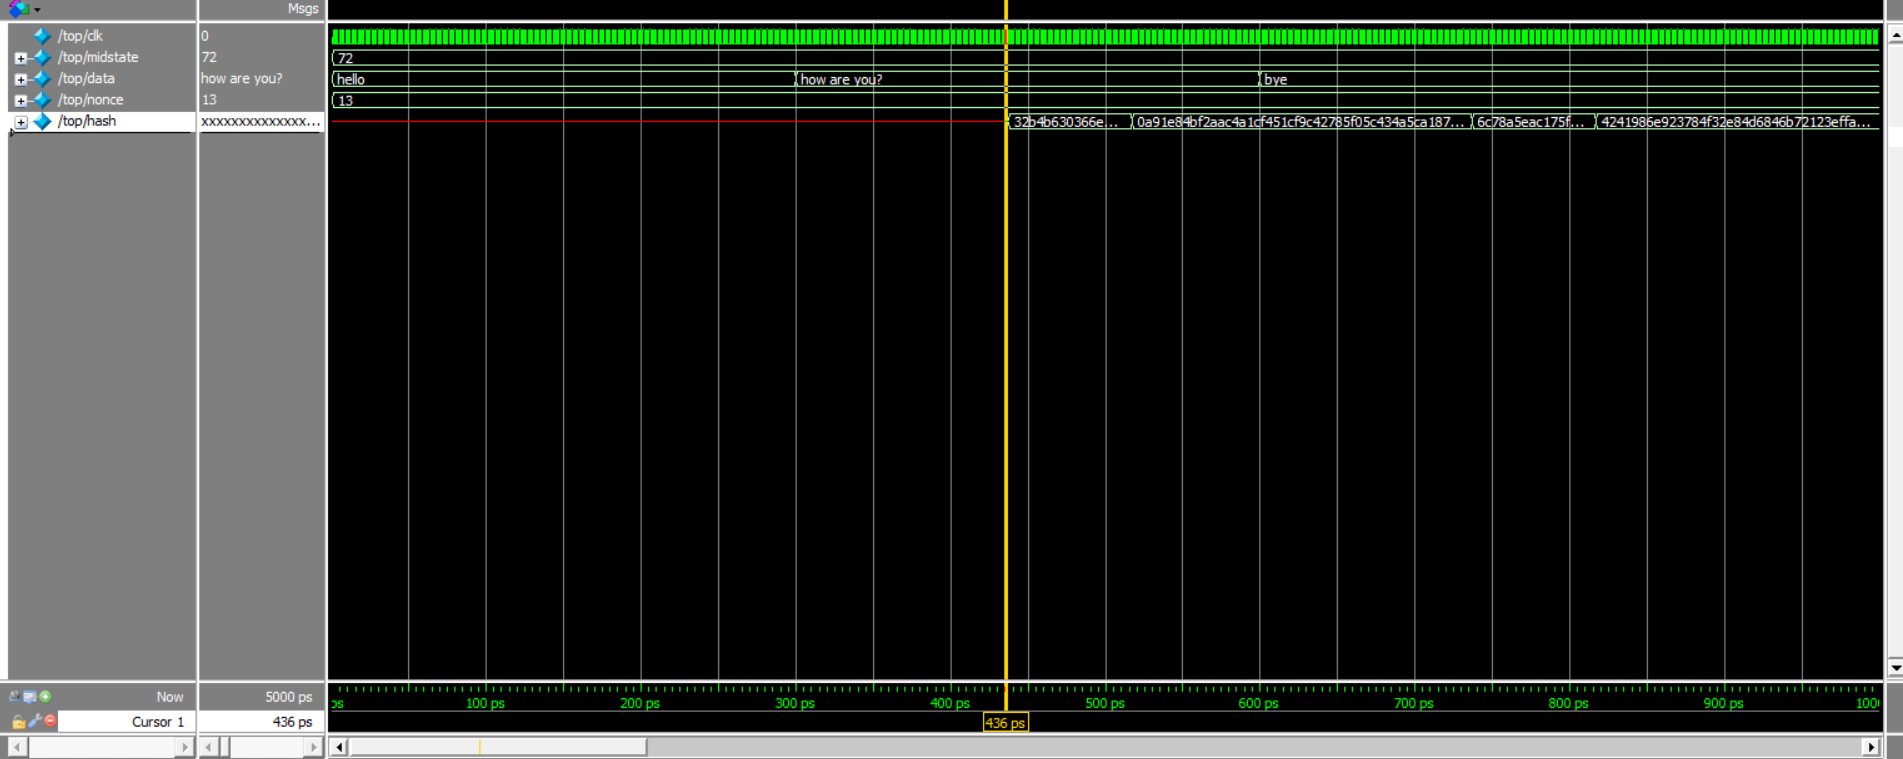
\includegraphics[width = \textwidth]{figs/simulation/1.png}
	\caption{شبیه‌سازی با \lr{Testbench}}
	\label{simulation_1}
\end{figure}

\subsection{جدول ورودی‌ها و خروجی‌های  Testbench}
\lr{
	\begin{table}[H]
		\resizebox{\textwidth}{!}{%
			\begin{tabular}{@{}llll@{}}
				\toprule
				Midstate & Nonce   & Data                                    & Time (clk)  \\ \midrule
				0        & 0       & 0                                       & 1000 - 0    \\
				96'd456  & 32'd453 & 512'd12345609823                        & 2000 - 1000 \\
				96'd456  & 32'd453 & 512'd7659432094555543122297600000000654 & End - 2000  \\ \bottomrule
			\end{tabular}%
		}
		\rl{
			\caption{مقادیر ورودی‌ها و زمان }}
		\label{table_input}
	\end{table}}

\lr{
	\begin{table}[H]
		\resizebox{\textwidth}{!}{%
			\begin{tabular}{@{}ll@{}}
				\toprule
				Hash                                                                                        \\ \midrule
				\begin{tabular}[c]{@{}l@{}}ab5283d68df053ac62d053789d4b45b81a02c959d7cab97fc43451166351f117 \\ f949fe918475f762ba80567046338211461648316d4432e6c505edc3b5ee6ff5\end{tabular} & 1217 - 433        \\
				\begin{tabular}[c]{@{}l@{}}dd477bfb0f07e299560b050c7aedb947bad77571f9a7d886a06f197a55f7946b \\ 8a9cecbb948a5478380168f8bfaf8e6d7d828459564973272b18cdf99d0234f2\end{tabular} & 1436 - 1217       \\
				\begin{tabular}[c]{@{}l@{}}0c0dea4dfd9994c6eb97f500589565239347be8a5b2e4ce4832c6cc9095baa51 \\ bf2bdde45ef619f4086e71e7d86f637314357e6d20632c31612f5424644cc223\end{tabular} & 2217 - 1436       \\
				\begin{tabular}[c]{@{}l@{}}6d383e0cceb223c20c45b816a165072ad200b8091682e8e5c31295ee62ca3719 \\ afbd493a4b85859d1cbe08d98bf01e66be18f3d3536987eeef06cc7965851bf8\end{tabular} & 2437 - 2217       \\
				\begin{tabular}[c]{@{}l@{}}6b722c1b1fb150c850e02ee44e03a447401ca4ac3cde4de6eb95b2e853d0d34b \\ 53583685f4b21f9b98229734756d7b835e46c2f589e461ab7c3177fb7e572b64\end{tabular} & End - 2437        \\ \bottomrule
			\end{tabular}%
		}
		\rl{
			\caption{مقادیر درهم‌سازی و زمان }}
		\label{table_hash}
	\end{table}}

\section{اجرا و تحلیل کد نرم‌افزاری (مدل طلایی)}
به همراه پروژه کد C الگوریتم Skein نیز به عنوان مدل طلایی ارائه شد، در ادامه مختصرا کد C مدل طلایی را تحلیل می‌کنیم.
\subsection{تحلیل کد C}
تابع $skeinhash$ با گرفتن ورودی $data$ که به صورت آرایه ای از $unsigned char$  و $output$ که به صورت آرایه‌ای از  $uint8\_t$ میباشد شروع می کند.با فراخواندن $sph\_skein512\_init$ که ورودی از جنس $sph\_skein\_big-contex$ می گیرد و سپس $sph\_skein512$ که ورودی $sph\_skein\_big-contex$ و داده و طول داده را می گیرد و در آخر $sph\_skein512\_close$ که خروجی و $sph\_skein\_big-context$ را به عنوان ورودی دارد کار خود را پایان می دهد و نتیجه را در آرایه خروجی به طول ۳۲ کپی می‌کند.\\
	در ابتدا $sph\_skein\_big-context$ بررسی می شود:
	زمینه ای برای محاسبه ی اسکین شامل مقادیر واسطه و بخشی از داده از آخرین بلوک وارد شده است.
\begin{ccode}
#ifndef DOXYGEN_IGNORE
	unsigned char buf[64];    /* first field, for alignment */
	size_t ptr; 
	sph_u64 h0, h1, h2, h3, h4, h5, h6, h7;
	sph_u64 bcount;
#endif
} sph_skein_big_context;
\end{ccode}
\begin{itemize}
\item
$buf$\\ آرایه ای به طول ۶۴ که بخش به بخش داداه را در خود ذخیره می‌کند و روی آن پردازش انجام می‌شود.
\item
$ptr$\\ سایز بخش اشغال شده بافر
\item
$h0..h7$\\
 \item
 تعداد بلاک های داده\\$bcount$
\end{itemize}
تابع $skein\_big\_init$ مقادیر  $sph\_skein\_big-context$ که از این به بعد از آن به اختصار $ctx$ یاد میشود را مقدار دهی اولیه کرده و تمامی مقادیر آن را به جز بافر صفر می‌گذارد.\\
تابع $sph\_skein512$ بخش اصلی محاسبات را به عهده دارد.اگر سایز بافر $ctx$ خالی مانده بیشتر از طول داده باشد داده در آن کپی می‌شود.\\
سپس مقادیر $ctx$ توسط تابع $READ\_STATE\_BIG$ به روز رسانی می‌شوند و با مشخص کردن مقدار $first$ که بعدتر از آن استفاده میکند و برابر با متغیر$ first$ در $UBI$  می‌باشد با استفاده از $bcount$ زمینه که در ابتدا برابر با $0$ است ،وارد لوپ محاسبه می‌شود.\\
اگر بافر پر شده باشد، $bcount$ به علاوه یک شده و $first$  و $ptr$ صفر می‌شوند. تابع $UBI\_BIG$ با ورودی $96+first$ و $0$ فراخوانی می‌شود که همان
\lr{ The Unique Block Iteration (UBI) chaining mode}
 است که یک مقدار زنجیره ای ورودی را با یک رشته ورودی با طول اختیاری ترکیب می کند و خروجی با طول ثابت را تولید می کند.\\
.بلوک های پیام $M0$ و $M1$ و …و $M7$ هرکدام گنجایش 64 بیت داده را دارند که به ترتیب توسط  بافر$ ctx$ پر می‌شوند.\\
 مقدار $p0…p7$ مربوط به threefish که متن ساده، یک رشته از بایت های با طولی برابر با کلید، است برابر $m0..m7$ قرار می‌گیرد.\\
دو متغیر $t0$ و $t1(threefish tweak)$ با استفاده از $bcount$  که متعلق به $ctx$ است و ورودی های تابع  $UBI\_BIG$ محاسبه میشوند و تابع $TFBIG\_KINIT$با ورودی های $h0 …h7 $مربوط به $ctx$ و $t0$ و $t1$ که قبلتر محاسبه شد فراخوانی میشود که با استفاده از آن و $TFBIG\_ADDKEY$ که با هم نقش  threefish اسکین را به عهده دارند $h0..h7$ مقدار دهی میشوند.به طوری که $hn = mn \textasciicircum pn$.\\
 و این مرحله تا وقتی داده ای که در بافر نرفته باقی  مانده ادامه دارد و سپس تمامی مقادیر $ctx$ در آن نوشته میشوند.(به جز بافر)\\
 تابع  $skein\_big\_close$ چند بیت اضافی (0 تا 7) را به محاسبات فعلی اضافه میکند.خروجی را در بافر ارائه شده میریزد و به پردازش خاتمه میدهد. زمینه یا $ctx$ به طور خودکار دوباره مقدار دهی اولیه می‌شود.ورودی این تابع به جز زمینه و آرایه‌ی خروجی،تعداد بیت های اضافه $n$ و خود بیت های اضافه $ub $میباشد که خود تابع دو ورودی آخر را مشخص می‌کند.اگر $n $صفر نباشد مقدار $x$ ای با استفاده از این دو تولید میشود که$ sph\_skein512$ آن فراخوانی میشود.در این مرحله، اگر $ptr == 0$ یعنی پیام خالی است؛ در غیر این صورت، بین 1 تا 64 بایت وجود دارد که هنوز پردازش نشده اند. در هر صورت بافر باید به یک بلوک کامل پر شده با صفر تبدیل شود(مشخصه Skein می گوید که پیام خالی پوشیده شده است تا حداقل یک بلوک برای پردازش وجود داشته باشد).
  هنگامی که این بلوک پردازش شده است، این فرآیند دوباره با بلوک پر از صفر، برای خروجی (آن بلوک encoding "0"، بیش از 8 بایت و سپس با صفر پر شده) انجام می شود.


\end{document}
